\documentclass[twoside]{book}

% Packages required by doxygen
\usepackage{fixltx2e}
\usepackage{calc}
\usepackage{doxygen}
\usepackage[export]{adjustbox} % also loads graphicx
\usepackage{graphicx}
\usepackage[utf8]{inputenc}
\usepackage{makeidx}
\usepackage{multicol}
\usepackage{multirow}
\PassOptionsToPackage{warn}{textcomp}
\usepackage{textcomp}
\usepackage[nointegrals]{wasysym}
\usepackage[table]{xcolor}

% NLS support packages
Portuguese
% Font selection
\usepackage[T1]{fontenc}
\usepackage[scaled=.90]{helvet}
\usepackage{courier}
\usepackage{amssymb}
\usepackage{sectsty}
\renewcommand{\familydefault}{\sfdefault}
\allsectionsfont{%
  \fontseries{bc}\selectfont%
  \color{darkgray}%
}
\renewcommand{\DoxyLabelFont}{%
  \fontseries{bc}\selectfont%
  \color{darkgray}%
}
\newcommand{\+}{\discretionary{\mbox{\scriptsize$\hookleftarrow$}}{}{}}

% Page & text layout
\usepackage{geometry}
\geometry{%
  a4paper,%
  top=2.5cm,%
  bottom=2.5cm,%
  left=2.5cm,%
  right=2.5cm%
}
\tolerance=750
\hfuzz=15pt
\hbadness=750
\setlength{\emergencystretch}{15pt}
\setlength{\parindent}{0cm}
\setlength{\parskip}{3ex plus 2ex minus 2ex}
\makeatletter
\renewcommand{\paragraph}{%
  \@startsection{paragraph}{4}{0ex}{-1.0ex}{1.0ex}{%
    \normalfont\normalsize\bfseries\SS@parafont%
  }%
}
\renewcommand{\subparagraph}{%
  \@startsection{subparagraph}{5}{0ex}{-1.0ex}{1.0ex}{%
    \normalfont\normalsize\bfseries\SS@subparafont%
  }%
}
\makeatother

% Headers & footers
\usepackage{fancyhdr}
\pagestyle{fancyplain}
\fancyhead[LE]{\fancyplain{}{\bfseries\thepage}}
\fancyhead[CE]{\fancyplain{}{}}
\fancyhead[RE]{\fancyplain{}{\bfseries\leftmark}}
\fancyhead[LO]{\fancyplain{}{\bfseries\rightmark}}
\fancyhead[CO]{\fancyplain{}{}}
\fancyhead[RO]{\fancyplain{}{\bfseries\thepage}}
\fancyfoot[LE]{\fancyplain{}{}}
\fancyfoot[CE]{\fancyplain{}{}}
\fancyfoot[RE]{\fancyplain{}{\bfseries\scriptsize Gerado por Doxygen }}
\fancyfoot[LO]{\fancyplain{}{\bfseries\scriptsize Gerado por Doxygen }}
\fancyfoot[CO]{\fancyplain{}{}}
\fancyfoot[RO]{\fancyplain{}{}}
\renewcommand{\footrulewidth}{0.4pt}
\renewcommand{\chaptermark}[1]{%
  \markboth{#1}{}%
}
\renewcommand{\sectionmark}[1]{%
  \markright{\thesection\ #1}%
}

% Indices & bibliography
\usepackage{natbib}
\usepackage[titles]{tocloft}
\setcounter{tocdepth}{3}
\setcounter{secnumdepth}{5}
\makeindex

% Hyperlinks (required, but should be loaded last)
\usepackage{ifpdf}
\ifpdf
  \usepackage[pdftex,pagebackref=true]{hyperref}
\else
  \usepackage[ps2pdf,pagebackref=true]{hyperref}
\fi
\hypersetup{%
  colorlinks=true,%
  linkcolor=blue,%
  citecolor=blue,%
  unicode%
}

% Custom commands
\newcommand{\clearemptydoublepage}{%
  \newpage{\pagestyle{empty}\cleardoublepage}%
}

\usepackage{caption}
\captionsetup{labelsep=space,justification=centering,font={bf},singlelinecheck=off,skip=4pt,position=top}

%===== C O N T E N T S =====

\begin{document}

% Titlepage & ToC
\hypersetup{pageanchor=false,
             bookmarksnumbered=true,
             pdfencoding=unicode
            }
\pagenumbering{alph}
\begin{titlepage}
\vspace*{7cm}
\begin{center}%
{\Large Projeto Final -\/ Computação gráfica -\/ U\+F\+RN 2019 }\\
\vspace*{1cm}
{\large Gerado por Doxygen 1.8.13}\\
\end{center}
\end{titlepage}
\clearemptydoublepage
\pagenumbering{roman}
\tableofcontents
\clearemptydoublepage
\pagenumbering{arabic}
\hypersetup{pageanchor=true}

%--- Begin generated contents ---
\chapter{Índice da hierarquia}
\section{Hierarquia de classes}
Esta lista de heranças está organizada, dentro do possível, por ordem alfabética\+:\begin{DoxyCompactList}
\item \contentsline{section}{Camera}{\pageref{classCamera}}{}
\item \contentsline{section}{Image\+R\+G\+Bf}{\pageref{classImageRGBf}}{}
\item \contentsline{section}{Light\+Source}{\pageref{classLightSource}}{}
\item \contentsline{section}{Material}{\pageref{classMaterial}}{}
\item \contentsline{section}{Object}{\pageref{classObject}}{}
\begin{DoxyCompactList}
\item \contentsline{section}{Plane}{\pageref{classPlane}}{}
\item \contentsline{section}{Sphere}{\pageref{classSphere}}{}
\end{DoxyCompactList}
\item \contentsline{section}{Ray\+Tracer}{\pageref{classRayTracer}}{}
\item \contentsline{section}{Viewer\+Data}{\pageref{classViewerData}}{}
\item \contentsline{section}{World}{\pageref{classWorld}}{}
\end{DoxyCompactList}

\chapter{Índice dos componentes}
\section{Lista de componentes}
Lista de classes, estruturas, uniões e interfaces com uma breve descrição\+:\begin{DoxyCompactList}
\item\contentsline{section}{\hyperlink{classCamera}{Camera} }{\pageref{classCamera}}{}
\item\contentsline{section}{\hyperlink{classImageRGBf}{Image\+R\+G\+Bf} }{\pageref{classImageRGBf}}{}
\item\contentsline{section}{\hyperlink{classLightSource}{Light\+Source} }{\pageref{classLightSource}}{}
\item\contentsline{section}{\hyperlink{classMaterial}{Material} }{\pageref{classMaterial}}{}
\item\contentsline{section}{\hyperlink{classObject}{Object} }{\pageref{classObject}}{}
\item\contentsline{section}{\hyperlink{classPlane}{Plane} }{\pageref{classPlane}}{}
\item\contentsline{section}{\hyperlink{classRayTracer}{Ray\+Tracer} }{\pageref{classRayTracer}}{}
\item\contentsline{section}{\hyperlink{classSphere}{Sphere} }{\pageref{classSphere}}{}
\item\contentsline{section}{\hyperlink{classViewerData}{Viewer\+Data} }{\pageref{classViewerData}}{}
\item\contentsline{section}{\hyperlink{classWorld}{World} }{\pageref{classWorld}}{}
\end{DoxyCompactList}

\chapter{Documentação da classe}
\hypertarget{classCamera}{}\section{Referência à classe Camera}
\label{classCamera}\index{Camera@{Camera}}
\subsection*{Atributos Públicos}
\begin{DoxyCompactItemize}
\item 
\mbox{\Hypertarget{classCamera_a56ecb917a35453503d0b162bc9602bd2}\label{classCamera_a56ecb917a35453503d0b162bc9602bd2}} 
Vec {\bfseries pos}
\item 
\mbox{\Hypertarget{classCamera_a39af9b8f99ed7a507d08be930b9ca691}\label{classCamera_a39af9b8f99ed7a507d08be930b9ca691}} 
Vec {\bfseries lookat}
\item 
\mbox{\Hypertarget{classCamera_a4a24ba3577fd873d760cb22291d45c4e}\label{classCamera_a4a24ba3577fd873d760cb22291d45c4e}} 
Vec {\bfseries vup}
\end{DoxyCompactItemize}


A documentação para esta classe foi gerada a partir do seguinte ficheiro\+:\begin{DoxyCompactItemize}
\item 
/home/gabriel/workarea/raytracing/libsrc/raytracer/viewerdata/viewerdata.\+h\end{DoxyCompactItemize}

\hypertarget{classImageRGBf}{}\section{Referência à classe Image\+R\+G\+Bf}
\label{classImageRGBf}\index{Image\+R\+G\+Bf@{Image\+R\+G\+Bf}}
\subsection*{Membros públicos}
\begin{DoxyCompactItemize}
\item 
\mbox{\Hypertarget{classImageRGBf_acee10672e885f5e0f3a9db7bf24059d2}\label{classImageRGBf_acee10672e885f5e0f3a9db7bf24059d2}} 
{\bfseries Image\+R\+G\+Bf} (uint width, uint height)
\item 
\mbox{\Hypertarget{classImageRGBf_a896e20a0b686b16673ca194deca69f41}\label{classImageRGBf_a896e20a0b686b16673ca194deca69f41}} 
void {\bfseries set\+Color} (uint i, uint j, const Vec \&color)
\item 
\mbox{\Hypertarget{classImageRGBf_aeca1409e7489d02a45961a595de3ba61}\label{classImageRGBf_aeca1409e7489d02a45961a595de3ba61}} 
float \& {\bfseries operator()} (uint i, uint j, uint k)
\item 
\mbox{\Hypertarget{classImageRGBf_acee10672e885f5e0f3a9db7bf24059d2}\label{classImageRGBf_acee10672e885f5e0f3a9db7bf24059d2}} 
{\bfseries Image\+R\+G\+Bf} (uint width, uint height)
\item 
\mbox{\Hypertarget{classImageRGBf_a896e20a0b686b16673ca194deca69f41}\label{classImageRGBf_a896e20a0b686b16673ca194deca69f41}} 
void {\bfseries set\+Color} (uint i, uint j, const Vec \&color)
\item 
\mbox{\Hypertarget{classImageRGBf_ab50aa22791513e10ed01d2a970dd7d31}\label{classImageRGBf_ab50aa22791513e10ed01d2a970dd7d31}} 
float \& {\bfseries operator()} (uint i, uint j, uint k)
\end{DoxyCompactItemize}
\subsection*{Atributos Públicos}
\begin{DoxyCompactItemize}
\item 
\mbox{\Hypertarget{classImageRGBf_a5ab048f770e190a418a935b772ad809d}\label{classImageRGBf_a5ab048f770e190a418a935b772ad809d}} 
float $\ast$ {\bfseries data}
\item 
\mbox{\Hypertarget{classImageRGBf_a6ec173fcc2dfe9df78bd365418f42db4}\label{classImageRGBf_a6ec173fcc2dfe9df78bd365418f42db4}} 
uint {\bfseries width}
\item 
\mbox{\Hypertarget{classImageRGBf_a05f92bf07d095d1d00594282758bfc60}\label{classImageRGBf_a05f92bf07d095d1d00594282758bfc60}} 
uint {\bfseries height}
\end{DoxyCompactItemize}


A documentação para esta classe foi gerada a partir dos seguintes ficheiros\+:\begin{DoxyCompactItemize}
\item 
/home/gabriel/workarea/raytracing/include/raytracer.\+h\item 
/home/gabriel/workarea/raytracing/libsrc/raytracer/raytracer.\+cpp\end{DoxyCompactItemize}

\hypertarget{classLightSource}{}\section{Referência à classe Light\+Source}
\label{classLightSource}\index{Light\+Source@{Light\+Source}}
\subsection*{Membros públicos}
\begin{DoxyCompactItemize}
\item 
\mbox{\Hypertarget{classLightSource_a0caf4cbfb23525a87d4918e73c440e0e}\label{classLightSource_a0caf4cbfb23525a87d4918e73c440e0e}} 
{\bfseries Light\+Source} (Vec p, Vec c)
\end{DoxyCompactItemize}
\subsection*{Atributos Públicos}
\begin{DoxyCompactItemize}
\item 
\mbox{\Hypertarget{classLightSource_aab1890cf682612a28d12d8323e94db39}\label{classLightSource_aab1890cf682612a28d12d8323e94db39}} 
Vec {\bfseries pos}
\item 
\mbox{\Hypertarget{classLightSource_a6438b2de502fb184234d5e70f5d0be49}\label{classLightSource_a6438b2de502fb184234d5e70f5d0be49}} 
Vec {\bfseries color}
\end{DoxyCompactItemize}


A documentação para esta classe foi gerada a partir do seguinte ficheiro\+:\begin{DoxyCompactItemize}
\item 
/home/gabriel/workarea/raytracing/libsrc/raytracer/object/object.\+h\end{DoxyCompactItemize}

\hypertarget{classMaterial}{}\section{Referência à classe Material}
\label{classMaterial}\index{Material@{Material}}
\subsection*{Membros públicos}
\begin{DoxyCompactItemize}
\item 
\mbox{\Hypertarget{classMaterial_a49440e5c169730bbbe452f64a231294d}\label{classMaterial_a49440e5c169730bbbe452f64a231294d}} 
{\bfseries Material} (const float \&ks, const \&float kd, const float \&n\+\_\+shiny, const Vec \&color)
\end{DoxyCompactItemize}
\subsection*{Membros públicos estáticos}
\begin{DoxyCompactItemize}
\item 
\mbox{\Hypertarget{classMaterial_ab6a3ae3a1ec4abc634d6bdddb9a5b63f}\label{classMaterial_ab6a3ae3a1ec4abc634d6bdddb9a5b63f}} 
static \hyperlink{classMaterial}{Material} {\bfseries rand\+Material} ()
\end{DoxyCompactItemize}
\subsection*{Atributos Públicos}
\begin{DoxyCompactItemize}
\item 
\mbox{\Hypertarget{classMaterial_ae79b3f2a118fa5d47e030396cf1bb9c2}\label{classMaterial_ae79b3f2a118fa5d47e030396cf1bb9c2}} 
float {\bfseries ks}
\item 
\mbox{\Hypertarget{classMaterial_a2076127f606e22d9fe55b6be6ca519d1}\label{classMaterial_a2076127f606e22d9fe55b6be6ca519d1}} 
float {\bfseries kd}
\item 
\mbox{\Hypertarget{classMaterial_a6bee0b3a16931951becaa33699621983}\label{classMaterial_a6bee0b3a16931951becaa33699621983}} 
float {\bfseries n\+\_\+shiny}
\item 
\mbox{\Hypertarget{classMaterial_a9582259ac6757247d65a4cb7d08708eb}\label{classMaterial_a9582259ac6757247d65a4cb7d08708eb}} 
Vec {\bfseries color}
\end{DoxyCompactItemize}


A documentação para esta classe foi gerada a partir do seguinte ficheiro\+:\begin{DoxyCompactItemize}
\item 
/home/gabriel/workarea/raytracing/libsrc/raytracer/object/object.\+h\end{DoxyCompactItemize}

\hypertarget{classObject}{}\section{Referência à classe Object}
\label{classObject}\index{Object@{Object}}


Diagrama de heranças da classe Object\nopagebreak
\begin{figure}[H]
\begin{center}
\leavevmode
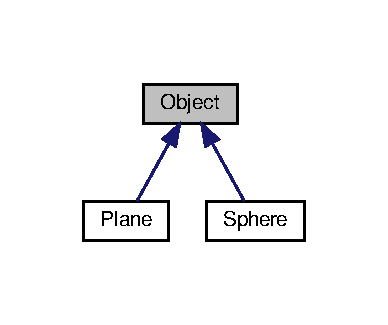
\includegraphics[width=186pt]{classObject__inherit__graph}
\end{center}
\end{figure}


Diagrama de colaboração para Object\+:\nopagebreak
\begin{figure}[H]
\begin{center}
\leavevmode
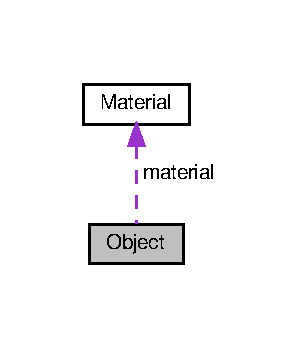
\includegraphics[width=144pt]{classObject__coll__graph}
\end{center}
\end{figure}
\subsection*{Membros públicos}
\begin{DoxyCompactItemize}
\item 
\mbox{\Hypertarget{classObject_add13c54b5bd59c48f75644753731ff12}\label{classObject_add13c54b5bd59c48f75644753731ff12}} 
{\bfseries Object} (\hyperlink{classMaterial}{Material} material, Vec pos)
\item 
\mbox{\Hypertarget{classObject_acd4358b792be07499816e6849e52bbe2}\label{classObject_acd4358b792be07499816e6849e52bbe2}} 
virtual bool {\bfseries intersect\+Point} (Vec line, Vec \&point)=0
\end{DoxyCompactItemize}
\subsection*{Atributos Públicos}
\begin{DoxyCompactItemize}
\item 
\mbox{\Hypertarget{classObject_a029376a01e31536d24013a5d65580184}\label{classObject_a029376a01e31536d24013a5d65580184}} 
Vec {\bfseries pos}
\item 
\mbox{\Hypertarget{classObject_a2f63d05a9a9264e1b6c388fa4bba4e91}\label{classObject_a2f63d05a9a9264e1b6c388fa4bba4e91}} 
\hyperlink{classMaterial}{Material} {\bfseries material}
\end{DoxyCompactItemize}


A documentação para esta classe foi gerada a partir do seguinte ficheiro\+:\begin{DoxyCompactItemize}
\item 
/home/gabriel/workarea/raytracing/libsrc/raytracer/object/object.\+h\end{DoxyCompactItemize}

\hypertarget{classPlane}{}\section{Referência à classe Plane}
\label{classPlane}\index{Plane@{Plane}}


Diagrama de heranças da classe Plane\nopagebreak
\begin{figure}[H]
\begin{center}
\leavevmode
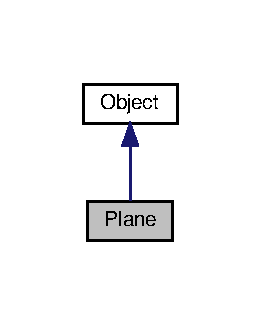
\includegraphics[width=125pt]{classPlane__inherit__graph}
\end{center}
\end{figure}


Diagrama de colaboração para Plane\+:\nopagebreak
\begin{figure}[H]
\begin{center}
\leavevmode
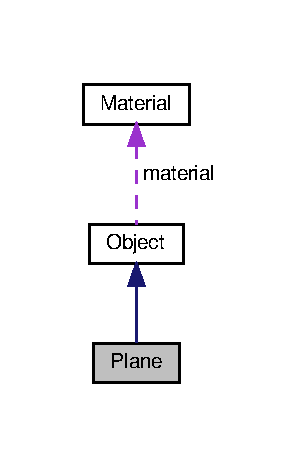
\includegraphics[width=144pt]{classPlane__coll__graph}
\end{center}
\end{figure}
\subsection*{Membros públicos}
\begin{DoxyCompactItemize}
\item 
\mbox{\Hypertarget{classPlane_a93e27a016a79fc07802a495e26737797}\label{classPlane_a93e27a016a79fc07802a495e26737797}} 
{\bfseries Plane} (\hyperlink{classMaterial}{Material} material, Vec pos, Vec normal)
\item 
\mbox{\Hypertarget{classPlane_a0458915a12d387dedf4e6cc723ef19f4}\label{classPlane_a0458915a12d387dedf4e6cc723ef19f4}} 
bool {\bfseries intersect\+Point} (Vec line, Vec \&point)
\end{DoxyCompactItemize}
\subsection*{Atributos Públicos}
\begin{DoxyCompactItemize}
\item 
\mbox{\Hypertarget{classPlane_a818fe2eba7bff65f6c47d6f83c9cc63f}\label{classPlane_a818fe2eba7bff65f6c47d6f83c9cc63f}} 
Vec {\bfseries normal}
\end{DoxyCompactItemize}


A documentação para esta classe foi gerada a partir do seguinte ficheiro\+:\begin{DoxyCompactItemize}
\item 
/home/gabriel/workarea/raytracing/libsrc/raytracer/object/object.\+h\end{DoxyCompactItemize}

\hypertarget{classRayTracer}{}\section{Referência à classe Ray\+Tracer}
\label{classRayTracer}\index{Ray\+Tracer@{Ray\+Tracer}}


Diagrama de colaboração para Ray\+Tracer\+:
\nopagebreak
\begin{figure}[H]
\begin{center}
\leavevmode
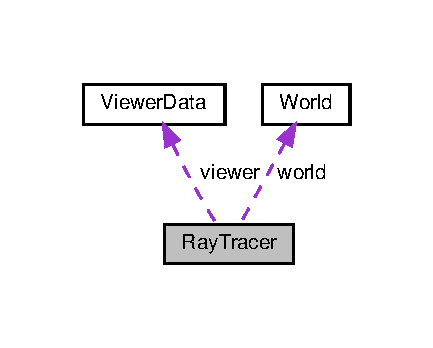
\includegraphics[width=208pt]{classRayTracer__coll__graph}
\end{center}
\end{figure}
\subsection*{Membros públicos}
\begin{DoxyCompactItemize}
\item 
\mbox{\Hypertarget{classRayTracer_aa4df800980bc0031eb6d15cf805feee9}\label{classRayTracer_aa4df800980bc0031eb6d15cf805feee9}} 
void {\bfseries ray\+Trace} (\hyperlink{classImageRGBf}{Image\+R\+G\+Bf} \&img, int num\+Refletion)
\item 
\mbox{\Hypertarget{classRayTracer_aa4df800980bc0031eb6d15cf805feee9}\label{classRayTracer_aa4df800980bc0031eb6d15cf805feee9}} 
void {\bfseries ray\+Trace} (\hyperlink{classImageRGBf}{Image\+R\+G\+Bf} \&img, int num\+Refletion)
\end{DoxyCompactItemize}
\subsection*{Atributos Públicos}
\begin{DoxyCompactItemize}
\item 
\mbox{\Hypertarget{classRayTracer_a2f48f14c213ea10dbd1fa4c804913f91}\label{classRayTracer_a2f48f14c213ea10dbd1fa4c804913f91}} 
\hyperlink{classWorld}{World} {\bfseries world}
\item 
\mbox{\Hypertarget{classRayTracer_adf5b36f3b4e1e61ccb5afebba1e095b7}\label{classRayTracer_adf5b36f3b4e1e61ccb5afebba1e095b7}} 
\hyperlink{classViewerData}{Viewer\+Data} {\bfseries viewer}
\end{DoxyCompactItemize}


A documentação para esta classe foi gerada a partir dos seguintes ficheiros\+:\begin{DoxyCompactItemize}
\item 
/home/gabriel/workarea/raytracing/include/raytracer.\+h\item 
/home/gabriel/workarea/raytracing/libsrc/raytracer/raytracer.\+cpp\end{DoxyCompactItemize}

\hypertarget{classSphere}{}\section{Referência à classe Sphere}
\label{classSphere}\index{Sphere@{Sphere}}


Diagrama de heranças da classe Sphere\nopagebreak
\begin{figure}[H]
\begin{center}
\leavevmode
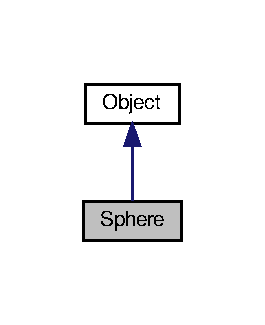
\includegraphics[width=127pt]{classSphere__inherit__graph}
\end{center}
\end{figure}


Diagrama de colaboração para Sphere\+:\nopagebreak
\begin{figure}[H]
\begin{center}
\leavevmode
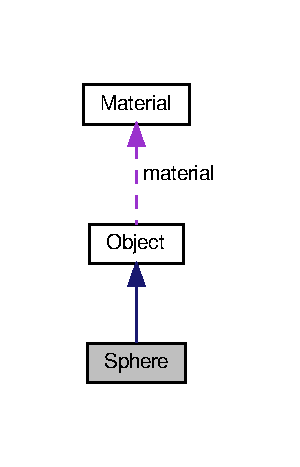
\includegraphics[width=144pt]{classSphere__coll__graph}
\end{center}
\end{figure}
\subsection*{Membros públicos}
\begin{DoxyCompactItemize}
\item 
\mbox{\Hypertarget{classSphere_a3cdbd5e616f29a25e11b2288623f4a27}\label{classSphere_a3cdbd5e616f29a25e11b2288623f4a27}} 
{\bfseries Sphere} (\hyperlink{classMaterial}{Material} material, Vec pos, float r)
\item 
\mbox{\Hypertarget{classSphere_aef46fad76354a361e9cd191169f0ee0b}\label{classSphere_aef46fad76354a361e9cd191169f0ee0b}} 
bool {\bfseries intersect\+Point} (Vec line, Vec \&point)
\end{DoxyCompactItemize}
\subsection*{Atributos Públicos}
\begin{DoxyCompactItemize}
\item 
\mbox{\Hypertarget{classSphere_a2b1b412591a00eb30cb012e444f7192d}\label{classSphere_a2b1b412591a00eb30cb012e444f7192d}} 
float {\bfseries r}
\end{DoxyCompactItemize}


A documentação para esta classe foi gerada a partir do seguinte ficheiro\+:\begin{DoxyCompactItemize}
\item 
/home/gabriel/workarea/raytracing/libsrc/raytracer/object/object.\+h\end{DoxyCompactItemize}

\hypertarget{classViewerData}{}\section{Referência à classe Viewer\+Data}
\label{classViewerData}\index{Viewer\+Data@{Viewer\+Data}}
\subsection*{Membros públicos}
\begin{DoxyCompactItemize}
\item 
\mbox{\Hypertarget{classViewerData_adb33c498d7487ec395b653fa6c6919e0}\label{classViewerData_adb33c498d7487ec395b653fa6c6919e0}} 
{\bfseries Projection} ()
\item 
\mbox{\Hypertarget{classViewerData_a3ee0f7787abc738bdb5e5a9230a9b43a}\label{classViewerData_a3ee0f7787abc738bdb5e5a9230a9b43a}} 
void {\bfseries pixel\+To\+World} (const int \&wx, const int \&wx, Vec \&pos\+World)
\item 
\mbox{\Hypertarget{classViewerData_a807be7d7ca8007b704042a1171dd4e31}\label{classViewerData_a807be7d7ca8007b704042a1171dd4e31}} 
void {\bfseries pixel\+Direction2\+Wolrd} (const int \&wx, const int \&wx, Vec \&versor)
\item 
\mbox{\Hypertarget{classViewerData_a03331984493c1546045dd937f16b36e9}\label{classViewerData_a03331984493c1546045dd937f16b36e9}} 
void {\bfseries set\+Window\+Size} (int win\+\_\+width, int win\+\_\+height)
\item 
\mbox{\Hypertarget{classViewerData_afae331d6cb58e5bec58ced3bdabf3013}\label{classViewerData_afae331d6cb58e5bec58ced3bdabf3013}} 
void {\bfseries set\+Camera} (const \hyperlink{classCamera}{Camera} \&camera)
\item 
\mbox{\Hypertarget{classViewerData_ac2e795bd6c13d03b5ed9e721c04eac0e}\label{classViewerData_ac2e795bd6c13d03b5ed9e721c04eac0e}} 
void {\bfseries set\+Pespective} (float angleP, float znear, float zfar)
\end{DoxyCompactItemize}


A documentação para esta classe foi gerada a partir do seguinte ficheiro\+:\begin{DoxyCompactItemize}
\item 
/home/gabriel/workarea/raytracing/libsrc/raytracer/viewerdata/viewerdata.\+h\end{DoxyCompactItemize}

\hypertarget{classWorld}{}\section{Referência à classe World}
\label{classWorld}\index{World@{World}}
\subsection*{Membros públicos}
\begin{DoxyCompactItemize}
\item 
\mbox{\Hypertarget{classWorld_a07fc4f8881889180e745a9843f331ffe}\label{classWorld_a07fc4f8881889180e745a9843f331ffe}} 
{\bfseries World} (Vec bg\+Color, float light\+Env)
\end{DoxyCompactItemize}
\subsection*{Atributos Públicos}
\begin{DoxyCompactItemize}
\item 
\mbox{\Hypertarget{classWorld_ab97841faf75338ea553d430cfc96a3e2}\label{classWorld_ab97841faf75338ea553d430cfc96a3e2}} 
std\+::list$<$ \hyperlink{classObject}{Object} $\ast$ $>$ {\bfseries objs}
\item 
\mbox{\Hypertarget{classWorld_abbefbccb58aaffa5cfe77a73d03e27db}\label{classWorld_abbefbccb58aaffa5cfe77a73d03e27db}} 
std\+::list$<$ \hyperlink{classLightSource}{Light\+Source} $>$ {\bfseries lights}
\item 
\mbox{\Hypertarget{classWorld_af8ca5773a58a6e7faee7beb824a1c5fc}\label{classWorld_af8ca5773a58a6e7faee7beb824a1c5fc}} 
Vec {\bfseries bg\+Color}
\item 
\mbox{\Hypertarget{classWorld_af618e742e01b9848f2355d027319cc74}\label{classWorld_af618e742e01b9848f2355d027319cc74}} 
float {\bfseries light\+Env}
\end{DoxyCompactItemize}


A documentação para esta classe foi gerada a partir do seguinte ficheiro\+:\begin{DoxyCompactItemize}
\item 
/home/gabriel/workarea/raytracing/libsrc/raytracer/world/world.\+h\end{DoxyCompactItemize}

%--- End generated contents ---

% Index
\backmatter
\newpage
\phantomsection
\clearemptydoublepage
\addcontentsline{toc}{chapter}{Índice}
\printindex

\end{document}
